\documentclass{article}
\usepackage[utf8]{inputenc}

\usepackage{latexsym}
\usepackage{float}
\usepackage[utf8]{inputenc}
\usepackage[catalan]{babel}
% \usepackage[english]{babel}
\usepackage{microtype}
\usepackage[hyphens]{url}
\usepackage{hyperref}
\usepackage{graphicx}
\usepackage[T1]{fontenc}
\usepackage{makeidx}
\usepackage{datetime}
\usepackage{multicol}
\usepackage{setspace}
\usepackage{enumerate}
\usepackage{booktabs}
\usepackage{listings}
\usepackage{color}
\usepackage{amsmath}
\usepackage{amssymb}
\usepackage[table,xcdraw]{xcolor}
\usepackage{graphicx}
\usepackage{listings}
\usepackage{hyperref}
\usepackage{vmargin}
\usepackage{wrapfig}
\usepackage{subfiles}
\usepackage{float}
\usepackage{amsmath}
\usepackage{amssymb}
\usepackage{tikz-cd}
\usepackage{multirow}
\usepackage{pgffor}
\usepackage{iflang}

%%%%%%%%%%%%%%%%%%%%%%%%%%%%%%%%%%%%%%%
%%%%%%%%%%%% UTIL COMMANDS %%%%%%%%%%%%  

\newcommand{\nc}{\newcommand}
\nc{\supindex}{\textsuperscript}

%%%%%%%%%%%%%%%%%%%%%%%%%%%%%%%%%%%%%%%
%%%%%%%%%%%%% CONFIG FILE %%%%%%%%%%%%%

\nc{\mytitle}{Anàlisis de fòrum anònim}
\nc{\mysubtitle}{Utilitzant Preferential Attachment sobre un pes inicial}
\nc{\authors}{Oriol Alàs Cercós}
\nc{\datetime}{30 d'octubre, 2020}
%15\supindex{th} of May, 2020}
\nc{\assignatura}{-}
\nc{\professorat}{Francesc Sebé}

% Per separar professors, utilitzar ','
% 	Ex: Maria, Joan, Pere

%%%%%%%%%%%%%%%%%%%%%%%%%%%%%%%%%%%%%%%
%%%%%%%%%%%%%  LANGUAGE   %%%%%%%%%%%%%

\newcommand{\tr}{\IfLanguageName{english}}

%%%%%%%%%%%%%%%%%%%%%%%%%%%%%%%%%%%%%%%
%%%%%%%%%%%%%%%%% MATH %%%%%%%%%%%%%%%%

\nc{\prob}[1]{P({#1})}
\nc{\probl}[2]{P({#1}|{#2})}

%%%%%%%%%%%%%%%%%%%%%%%%%%%%%%%%%%%%%%%
%%%%%%%%%%%%% TREE CREATOR %%%%%%%%%%%%

\setpapersize{A4}
\setmargins{2.5cm}  % margen izquierdo
{1.5cm}             % margen superior
{16.5cm}            % anchura del texto
{23.42cm}           % altura del texto
{10pt}              % altura de los encabezados
{1cm}               % espacio entre el texto y los encabezados
{0pt}               % altura del pie de página
{2cm}               % espaci\title{Determinització d'un autòmat finit}
\author{Oriol Alàs Cercós}
\date{29 d'Abril del 2019}

\def\contentsname{Índex}
\begin{document}
	

\begin{titlepage}
\begin{figure}[htb]
\begin{center}
	
\includegraphics[width=5cm]{imgs/UDL.png}
   	\vspace*{\stretch{1.0}}
   	\\
   	\medskip
   	\begin{center}
   		\noindent\rule{16.5cm}{0.4pt}
   		\medskip 
   		\\
      	\Huge\textbf{\mytitle}
      	\\\medskip 	\Large  \mysubtitle
      \\
      	
      	\noindent\rule{16.5cm}{0.4pt}
      	\\
      	\bigskip
      	\normalsize{\tr{Made by}{Realitzat per:}}
      	\\
      	\large\textit{\authors}
      	\\
      	\setlength{\parskip}{1em}
      	\normalsize{\tr{Delivery}{Data de lliurament:}}
      	\\
      	\large{\datetime}
   	\end{center}
   	\vspace*{\stretch{2.0}}
\end{center}
\end{figure}
\begin{flushright}
Universitat de Lleida
\\
Escola Politècnica Superior
\\
Grau en Enginyeria Informàtica
\\
\assignatura
\\
\medskip
\textbf{\tr{Professorate:}{Professorat:}}
\\
\foreach \n in \professorat{\n\\}
\end{flushright}
\thispagestyle{empty} 
\end{titlepage}
\tableofcontents
\thispagestyle{empty} 
%\newpage
\listoffigures
\listoftables
\thispagestyle{empty}
\newpage
\section{Introducció}
Utilitzant un fòrum basat en signatura anònima i que no es pot enllaçar, la forma d’escollir el conjunt K de la signatura
ring pot afectar la privadesa dels usuaris. En aquesta memòria, s'intenta arribar a una forma d'escollir el conjunt de la signatura millor que la uniformement aleatòria, de manera que no suposi altres problemes de privacitat i anonimitat. És per aquest motiu, que primer s'ha optat per realitzar una comparació sobre la tria uniforme i la preferencial per, després, anar combinant diferents estratègies per tal de trobar millors resultats.
\\
\\
El codi del programa de simulació s'ha desenvolupat en \texttt{python3} i es pot trobar \href{https://github.com/sergisi/glowing-dollop}{aquí}. Els paràmetres del programa dependrà de cada diferent anàlisis i evolució del programa, doncs en diferents etapes es busquen punts diferents.
\subsection{Població}
Per tal de realitzar una població aproximada a la realitat, la distribució emprada ha estat Zipf, on hi ha un gran conjunt de membres que realitzen pocs missatges i un de petit, que en realitza molts, tal i com es mostra en la Figura \ref{fig:zipf-s13}. En totes les simulacions s'ha realitzat una població de 200 persones on el membre més participatiu té 15 missatges.
\begin{figure}[H] 
	\centering
	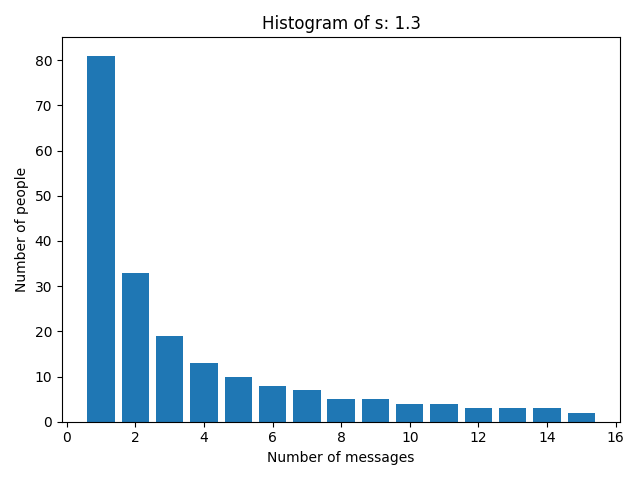
\includegraphics[width=10cm]{imgs/histogram-13.png}
	\caption{Histograma de la Distribució Zipf utilitzant $s=1.3$}
	\label{fig:zipf-s13}
\end{figure}
\section{Comparació entre selecció uniforme i tria preferent}
Per tal de realitzar la comparativa entre les dues opcions d'assignació, s'ha creat una classe que, un cop obtingudes totes les signatures i la llista d'autors per cada missatge, busca l'anonimitat per cada participant $P_i$, sent aquesta:
\[privacyScore(P_i)=K_i= \frac{N_i}{n_i} = \frac{n_i + r_i}{n_i}\]
\[n_i = {\textrm{nombre de missatges enviats per } P_i} \]
\[N_i = {\textrm{nombre de missatges assignats per } P_i}\]
Donades totes les puntuacions de privadesa dels diferents anells mitjançant una distribució Zipf específica, es calcula la mitjana d’un membre específic per comparar, en termes generals, la privadesa entre les diferents distribucions Zipf i els diferents mètodes de signatura de timbre.
\\
\\
Els paràmetres realitzats han estat:
\begin{itemize}
	\item Població:
	\begin{itemize}
		\item Distribució Zipf
		\item Nombre de participants: 200
		\item s: [1.3, 1.4, ..., 2.0]
		\item Nombre màxim de missatges d'un participant: 15
	\end{itemize}
	\item Signatura:
	\begin{itemize}
		\item K (ordre de l'anell): [3,12]
		\item Pes de la signatura: 1
	\end{itemize}
	\item Nombre de simulacions: 30
\end{itemize}
No obstant s'ha realitzat dades sobre diferents valors en la varible \textit{s}, s'ha cregut convenient només analitzar l'anonimitat en un cas, ja que són anàlegs.
\\
\\
S'ha trobat una lleugera millora sobre els membres més participatius en el Preferential Attachment. No obstant això, aquesta lleugera pujada podria ser a causa de possibles outliers molt significatius que distancien la privacitat general en aquests tipus de simulacions, ja que com poden veure en les taules \ref{tab:u13} i \ref{tab:p13}, l'anonimitat en participants poc actius es dispara.
\begin{table}[H]
\centering
\begin{tabular}{c|ccc}
K &1msm &5msm &15msm\\
\hline
3 & 10.4 & 2.34 & 1.4533\\
4 & 13.4 & 2.86 & 1.7533\\
5 & 17.7 & 3.76 & 1.9533\\
6 & 21.4 & 4.34 & 2.2133\\
7 & 24.8 & 4.82 & 2.4933\\
8 & 28.7 & 5.62 & 2.72\\
9 & 32.5 & 6.36 & 2.9267\\
10 & 36.7 & 7.16 & 3.2533\\
11 & 40.8 & 7.96 & 3.3867\\
12 & 44.9 & 8.84 & 3.5467\\
\hline
& 27.13 & 5.406 & 2.57\\
\end{tabular}
\caption{Uniformly random choice of Zipf distribution s:1.3}
\label{tab:s1.3}
\end{table}

\begin{table}[H]
\centering
\begin{tabular}{c|ccc}
K &1msm &5msm &15msm\\
\hline
3 & 10.4 & 2.34 & 1.4533\\
4 & 13.4 & 2.86 & 1.7533\\
5 & 17.7 & 3.76 & 1.9533\\
6 & 21.4 & 4.34 & 2.2133\\
7 & 24.8 & 4.82 & 2.4933\\
8 & 28.7 & 5.62 & 2.72\\
9 & 32.5 & 6.36 & 2.9267\\
10 & 36.7 & 7.16 & 3.2533\\
11 & 40.8 & 7.96 & 3.3867\\
12 & 44.9 & 8.84 & 3.5467\\
\hline
& 27.13 & 5.406 & 2.57\\
\end{tabular}
\caption{Uniformly random choice of Zipf distribution s:1.3}
\label{tab:s1.3}
\end{table}

Aquests outliers no són creats de manera aleatòria, sinó que el mateix mètode fa que els primers participants tinguin tant increment de pes de signatura sobre els altres que el seu nombre de signatures serà superior i, per tant, tindran beneficis sobre els altres en termes d'anonimitat.
\\\\
Per aquest motiu, la següent proposta de desenvolupament ha estat descobrir com reduir el pes de signatura al principi de la simulació per tal de no generar beneficis sobre els primers participants.
\section{Reducció del pes de signatura en inicis de la simulació}
Per tal de reduir aquest efecte inicial, s'ha realitzat un pes inicial uniforme per tots els participants de tal manera que la probabilitat de ser elegit en la següent signatura no sigui tan gran com abans. No obstant això, la probabilitat continua sent directament proporcional al nombre de missatges que ell envia.
\\\\
Per tal de veure la millora, s'ha realitzat una simulació amb 200 repeticiones per evitar casos no representatius. No obstant això, certs paràmetres del problema han estat especificats per tal que totes les repeticions representin un sol cas general. Les dades especificades han estat:
\begin{itemize}
	\item Població:
	\begin{itemize}	
		\item Distribució Zipf
		\item Nombre de participants: 200
		\item s: 1.3
		\item Nombre màxim de missatges d'un participant: 15
	\end{itemize}
	\item Signatura
	\begin{itemize}
		\item K: 6
		\item Pes de la signatura: [1-4]
		\item Pes inicial: [1-200]
	\end{itemize}
\item Nombre de simulacions: 200
\end{itemize}
S'ha buscat la mitjana i la mediana de la variable anonimitat per tal de buscar participants amb molta o poca prioritat (extrems). S'ha trobat més adhient buscar els participants amb més prioritat, doncs aquests, influïran a haver més participants amb poca anonimitat.
\\
\\
Gràcies a la Figura \ref{fig:weight1}, s'ha vist que els millors valors inicials estan entre 10 i 35. No obstant això, en valors propers a 10 (i sobtadament en algun altre valor) encara es troben missatges sense anonimitat. La mostra de resultats es poden trobar a la Taula \ref{tab1}. No obstant això, la no anonimitat es troba en pesos inicials baixos, sent el màxim 22.
\begin{figure}[H]
	\centering
	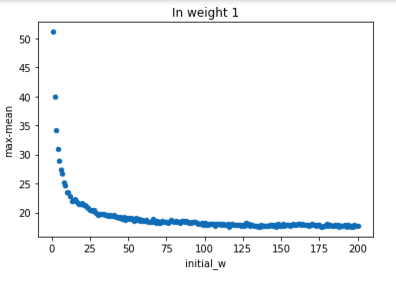
\includegraphics[width=7cm]{imgs/weight1.png}
	\label{fig:weight1}
	\caption{Gràfica de variació d'anonimitat entre el valor màxim i la mediana en cost de signatura=1.}
\end{figure}
\begin{figure}[H]
	\centering
	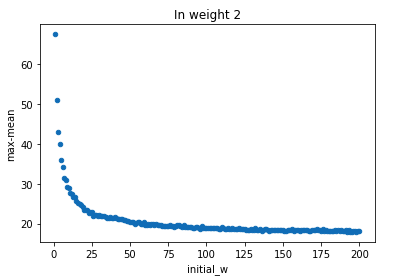
\includegraphics[width=7cm]{imgs/weight2.png}
	\label{fig:weight2}
	\caption{Gràfica de variació d'anonimitat entre el valor màxim i la mediana en cost de signatura=2.}
\end{figure}
\begin{figure}[H]
	\centering
	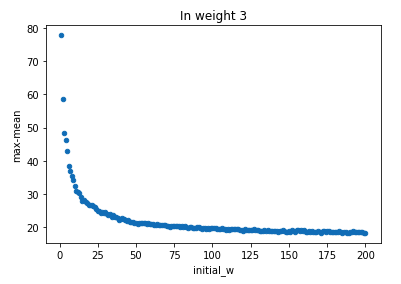
\includegraphics[width=7cm]{imgs/weight3.png}
	\label{fig:weight3}
	\caption{Gràfica de variació d'anonimitat entre el valor màxim i la mediana en cost de signatura=3.}
\end{figure}
\begin{figure}[H]
	\centering
	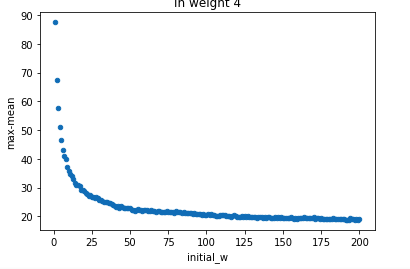
\includegraphics[width=7cm]{imgs/weight4.png}
	\label{fig:weight4}
	\caption{Gràfica de variació d'anonimitat entre el valor màxim i la mediana en cost de signatura=4.}
\end{figure}
\begin{table}[H]
	\centering
	\begin{tabular}{cc}
		initial weight & none-anonymity\\\hline
		8 & 0.010050 \\
		9 & 0.005025 \\
		10 & 0\\
		11& 0.010050\\
		12&0.005025 \\
		13&0.010050	\\
		14& 0.0 \\
		15&0.005025\\
		16& 0 \\
		17-20 & 0 \\
		21& 0 \\
		22 & 0.010050\\
		23& 0 \\
		24 - 200& 0 \\
	\end{tabular}
\label{tab1}
\caption{Taula de mitjana de no-anonimitat donat el pes inicial}
\end{table}
En aquest cas, ja és interessant trobar una relació entre el pes inicial, pes per signatura, ordre de l'anell i nombre de participants. Per tal d'intentar eliminar la no-anonimitat de participants i assegurar privacitat, es podria realitzar una funció de cost. No obstant això, el resultat que es busca no només és reduir la dispersió d'anonimitat sinó també si els participants més actius tenen millor anonimitat en aquesta nova estratègia d'elecció.
\section{Anonimitat entre participants}
Per realitzar un gràfic que busqui les diferents privacitats dels participants en rangs de pesos, s'ha hagut de crear noves simulacions. En aquest cas, els paràmetres han estat:
\begin{itemize}
	\item Població:
	\begin{itemize}	
		\item Distribució Zipf
		\item Nombre de participants: 200
		\item s: 1.3
		\item Nombre màxim de missatges d'un participant: 15
	\end{itemize}
	\item Signatura
	\begin{itemize}
		\item K: 8
		\item Pes de la signatura: 50
		\item Pes inicial: [1-150]
	\end{itemize}
	\item Nombre de simulacions: 100
\end{itemize}
Realitzant aquesta simulació, s'ha vist que el pes de signatura ha de ser un 20\% menor que el pes inicial:
\[w_s \leq 0.2 * w_i\]
En cas que sigui major, hi ha moltes més probabilitats que hi hagi un participant sense privacitat.
\\
\\
Per l'anàlisi, s'ha seleccionat 4 participants que envien 1, 5, 10 i 15 missatges per poder veure la seva anonimitat. A més, s'ha sobreposat la constant d'anonimitat en la selecció uniforme. Tal i com es pot veure a Figura \ref{fig:anonymity}, hi ha una petita tendència on la privacitat de diferents participants s'intenten acostar entre elles.
\begin{figure}[H]
	\centering
	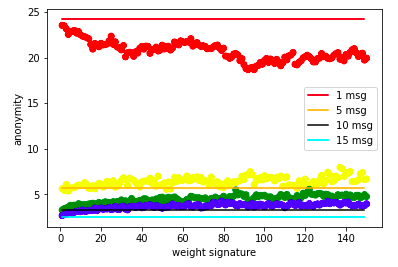
\includegraphics[width=8cm]{imgs/anonymity.png}
	\label{fig:anonymity}
	\caption{Gràfica d'anonimitat entre diferents participants en $p_i=50$ i $p_s\in[1,150]$}
\end{figure}
No obstant es vegui una baixada d'anonimitat en participants poc actius en rang on $p_s \in [80, 100]$, no es pot contemplar a punts majors $p_s \ge 10$, tenint en compte que el pes inicial és 50 i, que a mesura que augmenti el pes del Preferential Attachment, també augmenten les possibilitats de tenir participants sense anonimitat en la simulació. Aquest fet impossibilita una gran millora comparada amb la selecció uniforme. 
\\
\\
Com a conclusió d'aquesta anàlisi, tal i com es pot veure a la Taula \ref{tab:an_pa} es veu que no hi ha molta millora en els participants molt actius (només un 20\%)
\begin{table}[H]
	\centering
	\begin{tabular}{c|cccc}
		weight & person1 & person5 & person10 & person15\\\hline
		1.0 & 23.519231 & 5.636538 & 3.297115 & 2.691026\\
		2.0 & 23.471154 &5.451923 &3.441346 &2.791026\\
		9.0 & 22.846154 & 6.026923 & 3.988462 &3.189744
	\end{tabular}
\caption{Anonimitat en simulacions en $p_i=50$ utilitzant el PA amb pes inicial}
\label{tab:an_pa}
\end{table}
S'hauria de mirar si, creant una funció de pes de signatura es pot aconseguir un endarreriment de l'efecte inicial sense privar de privacitat en altres participants.
%\section{Conclusió}
%Tot el codi es troba a \url{https://github.com/sergisi/glowing-dollop/}
\end{document}
